\section{Esamų sistemų pertvarkymas}
Apibrėžus šablonus paketų skirstymui galima pradėti vertinti jų įtaką sistemai, juos pritaikant esamoms sistemoms.
Šio skyriaus tikslas - pasirinkti ir išnagrinėti kelias sistemas, pasitelkus paketų kokybės matus, bei bendrą sistemos struktūros analizę,
taip identifikuojant programiniam kodui būdingas problemas, rastas problemas išspręsti pritaikant aprašytus šablonus.
Atlikus pertvarkymus sistemose, dar kartą paskaičiuoti paketų kokybės matus,
taip gaunant įrodymus, ar gauti šablonai yra efektyvūs ir iš tiesų sprendžia
jiems priskirtas problemas.


\subsection{Sistemų pasirinkimas}
Sistemų pertvarkymui pasirinktos atviro kodo sistemos, kurių kodas yra viešai prietinamas \textit{github} platformoje.
Pasirinktos sistemos yra vidutinio dydžio, todėl nėra labai sudėtinga jas suprasti ir pertvarkyti, bet taip pat jos nėra
tokios paprastos, kad neturėtų sistemos dizaino problemų.
Pasirinktos sistemos yra skirtingo tipo projektai, taip užtikrinant didesnę problemų ivairovę ir objektyvesnius įvertinimus.
Per visą pasirinktų sistemų imtį yra sutinkamos visos aprašytos problemos, taip įvertinant visus aprašytus šablonus.

%\subsection{\textit{Leaf} sistema}
%\textbf{Leaf\footnote{\url{https://github.com/Meituan-Dianping/Leaf/tree/master}}} sistema, per \textit{http}
%protokolą teikianti aplikacijų programavimo sąsają unikalaus identifikatoriaus generavimui.
%Ši sistema užtikrina identifikatoriaus unikalų pasiskirstymą tarp skirtingų paskirstytų sistemų \angl{distributed systems},
%servisais orientuotoje \angl{service-oriented} architektūroje.
%Tai techninės programinės įrangos tipas, kuris naudojamas kitų taikomosios programinės įrangos sistemų.
%Sistema Leaf susideda iš dviejų modulių \textit{server} ir \textit{core}, šiame darbe dėmesys bus skirtas tik \textit{core} moduliui,
%kadangi \textit{server} modulis yra labai mažas
%ir paketų struktūra jame neatlieka esminio vaidmens.
%Prieš visus pakeitimus \textit{Leaf} sistemos, \textit{core} modulio paketų struktūra atrodo taip:
%\begin{figure}[H]
%    \centering
%    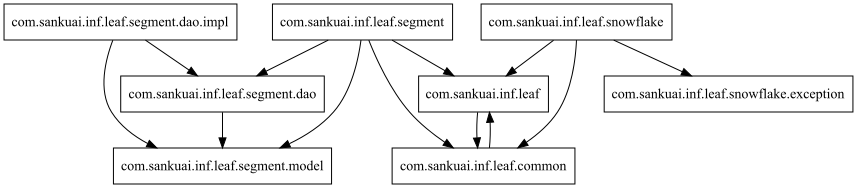
\includegraphics[scale=0.5]{img/leaf_packages_orig}
%    \caption{\textit{Leaf} sistemos \textit{core} modulio struktūra}
%    \label{img:leaf_packages_orig}
%\end{figure}
%
%\dirtree{%
%.1 {/}.
%.2 {common}.
%.2 {segment}.
%.3 {dao}.
%.4 {impl}.
%.3 {model}.
%.2 {snowflake}.
%.3 {exception}.
%}
%
%\begin{center}
%    \begin{tabular}{|c|c|c|c|c|c|c|}
%        \hline
%        Paketo vardas & \textit{N} & \textit{A} & \textit{E} & \textit{S} & \textit{A} & \textit{D} \\ [0.5ex]
%        \hline\hline
%        leaf.segment.dao.impl & 1 & 0 & 2 & 1.0 & 0.0 & 0.0 \\
%        \hline
%        leaf.segment & 1 & 0 & 4 & 1.0 & 0.0 & 0.0 \\
%        \hline
%        leaf.snowflake.exception & 3 & 1 & 0 & 0.0 & 0.0 & 1.0 \\
%        \hline
%        leaf.segment.model & 3 & 3 & 0 & 0.0 & 0.0 & 1.0 \\
%        \hline
%        leaf.segment.dao & 2 & 2 & 1 & 0.333 & 1.0 & 0.333 \\
%        \hline
%        leaf & 1 & 3 & 1 & 0.25 & 1.0 & 0.25 \\
%        \hline
%        leaf.common & 6 & 3 & 1 & 0.25 & 0.0 & 0.75 \\
%        \hline
%        leaf.snowflake & 2 & 0 & 3 & 1.0 & 0.0 & 0.0 \\
%        \hline
%    \end{tabular}
%    \begin{tabular}{|c|c|c|c|c|c|}
%        \hline
%        $\bar{N}$ & $\bar{A}$ & $\bar{E}$ & $\bar{S}$ & $\bar{A}$ & $\bar{D}$ \\ [0.5ex]
%        \hline\hline
%        2 & 2 & 2 & 0.479 & 0.25 & 0.417 \\
%        \hline
%    \end{tabular}
%\end{center}

%
%\subsection{\textit{HikariCP} sistema}
%
%\begin{figure}[H]
%    \centering
%    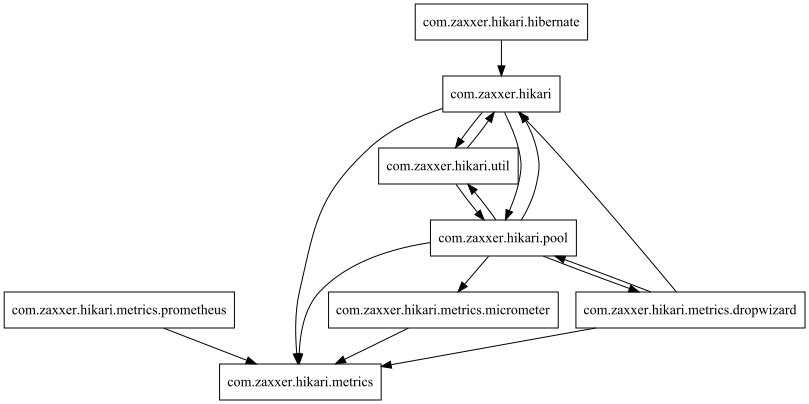
\includegraphics[scale=0.5]{img/hikari_packages_orig}
%    \caption{\textit{Hikari} sistemos struktūra}
%    \label{img:hikari_packages_orig}
%\end{figure}
%
%
%\dirtree{%
%    .1 {/} .
%    .2 {hikari}.
%    .3 {hibernate}.
%    .3 {metrics}.
%    .4 {dropwizard}.
%    .4 {micrometer}.
%    .4 {prometheus}.
%    .3 {pool}.
%    .3 {util}.
%}
%
%
%\begin{center}
%    \begin{tabular}{|c|c|c|c|c|c|c|}
%        \hline
%        Paketo vardas & \textit{N} & \textit{Af} & \textit{Ef} & \textit{S} & \textit{A} & \textit{D} \\ [0.5ex]
%        \hline\hline
%        com.zaxxer.hikari.metrics & 4 & 5 & 0 & 0.0 & 0.75 & 0.25 \\
%        \hline
%        com.zaxxer.hikari.metrics.prometheus & 5 & 0 & 1 & 1.0 & 0.0 & 0.0 \\
%        \hline
%        com.zaxxer.hikari & 6 & 4 & 3 & 0.429 & 0.5 & 0.071 \\
%        \hline
%        com.zaxxer.hikari.metrics.micrometer & 2 & 1 & 1 & 0.5 & 0.0 & 0.5 \\
%        \hline
%        com.zaxxer.hikari.metrics.dropwizard & 3 & 1 & 3 & 0.75 & 0.0 & 0.25 \\
%        \hline
%        com.zaxxer.hikari.pool & 12 & 3 & 5 & 0.625 & 0.583 & 0.208 \\
%        \hline
%        com.zaxxer.hikari.hibernate & 2 & 0 & 1 & 1.0 & 0.0 & 0.0 \\
%        \hline
%        com.zaxxer.hikari.util & 9 & 2 & 2 & 0.5 & 0.111 & 0.389 \\
%        \hline
%    \end{tabular}
%    \begin{tabular}{|c|c|c|c|c|c|}
%        \hline
%        $\bar{N}$ & $\bar{Af}$ & $\bar{Ef}$ & $\bar{S}$ & $\bar{A}$ & $\bar{D}$ \\ [0.5ex]
%        \hline\hline
%        5 & 2 & 2 & 0.601 & 0.243 & 0.209 \\
%        \hline
%    \end{tabular}
%\end{center}
%
%\subsection{\textit{chronicle map} sistema}
%\begin{center}
%    \begin{tabular}{|c|c|c|c|c|c|c|}
%        \hline
%        Paketo vardas & \textit{N} & \textit{A} & \textit{E} & \textit{S} & \textit{A} & \textit{D} \\ [0.5ex]
%        \hline\hline
%        net.openhft.chronicle.map.impl.stage.data.bytes & 2 & 3 & 3 & 0.5 & 0.0 & 0.5 \\
%        \hline
%        net.openhft.chronicle.map & 32 & 12 & 4 & 0.25 & 0.531 & 0.219 \\
%        \hline
%        net.openhft.chronicle.map.locks & 2 & 0 & 1 & 1.0 & 0.5 & 0.5 \\
%        \hline
%        net.openhft.chronicle.map.impl.ret & 2 & 3 & 1 & 0.25 & 1.0 & 0.25 \\
%        \hline
%        net.openhft.chronicle.map.impl.stage.data & 2 & 5 & 2 & 0.286 & 0.0 & 0.714 \\
%        \hline
%        net.openhft.chronicle.map.impl.stage.entry & 2 & 5 & 5 & 0.5 & 1.0 & 0.5 \\
%        \hline
%        net.openhft.chronicle.map.impl & 16 & 10 & 13 & 0.565 & 0.313 & 0.122 \\
%        \hline
%        net.openhft.chronicle.map.replication & 3 & 5 & 1 & 0.167 & 1.0 & 0.167 \\
%        \hline
%        net.openhft.chronicle.map.impl.stage.query & 9 & 2 & 7 & 0.778 & 0.667 & 0.445 \\
%        \hline
%        net.openhft.chronicle.map.impl.stage.map & 7 & 4 & 5 & 0.556 & 0.857 & 0.413 \\
%        \hline
%        net.openhft.chronicle.map.internal & 3 & 1 & 0 & 0.0 & 0.0 & 1.0 \\
%        \hline
%        net.openhft.chronicle.map.impl.stage.ret & 2 & 2 & 1 & 0.333 & 1.0 & 0.333 \\
%        \hline
%        net.openhft.chronicle.map.channel & 3 & 1 & 2 & 0.667 & 0.667 & 0.334 \\
%        \hline
%        net.openhft.chronicle.map.impl.stage.data.instance & 1 & 3 & 1 & 0.25 & 0.0 & 0.75 \\
%        \hline
%        net.openhft.chronicle.map.impl.stage.iter & 6 & 1 & 7 & 0.875 & 0.333 & 0.208 \\
%        \hline
%        net.openhft.chronicle.map.impl.stage.replication & 2 & 5 & 3 & 0.375 & 0.5 & 0.125 \\
%        \hline
%        net.openhft.chronicle.map.channel.internal & 1 & 1 & 2 & 0.667 & 0.0 & 0.333 \\
%        \hline
%        net.openhft.chronicle.map.impl.stage.input & 1 & 1 & 6 & 0.857 & 1.0 & 0.857 \\
%        \hline
%    \end{tabular}
%    \begin{tabular}{|c|c|c|c|c|c|}
%        \hline
%        $\bar{N}$ & $\bar{A}$ & $\bar{E}$ & $\bar{S}$ & $\bar{A}$ & $\bar{D}$ \\ [0.5ex]
%        \hline\hline
%        5 & 4 & 4 & 0.493 & 0.52 & 0.432 \\
%        \hline
%    \end{tabular}
%\end{center}
%
%
%\begin{figure}[H]
%    \centering
%    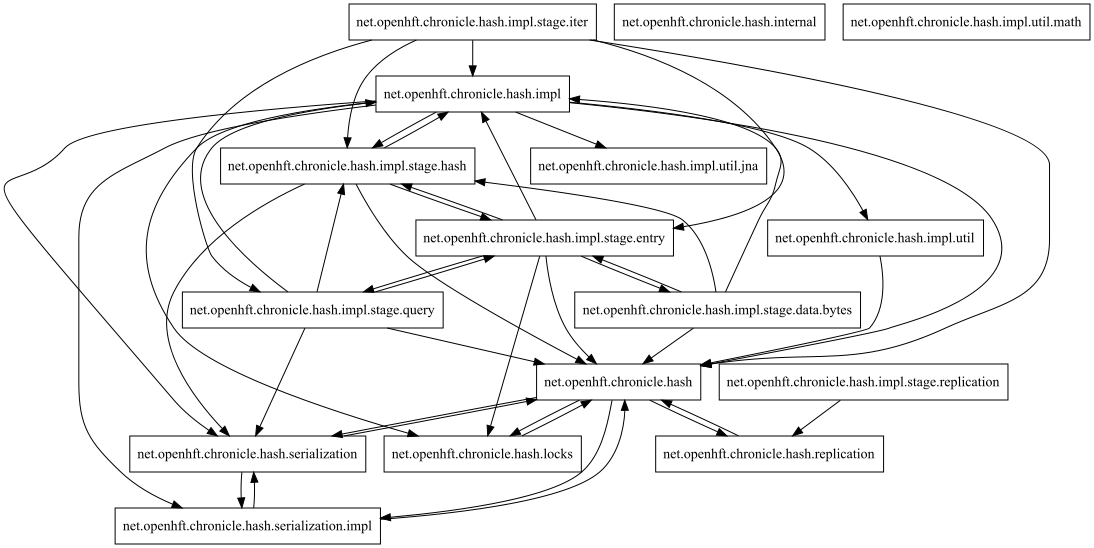
\includegraphics[scale=0.5]{img/open_hft_packages_orig}
%    \caption{\textit{Chronicle-map} sistemos struktūra}
%    \label{img:open_hft_packages_orig}
%\end{figure}
%
%\begin{center}
%    \begin{tabular}{|c|c|c|c|c|c|c|c|}
%        \hline
%        Paketo vardas & \textit{N} & \textit{Af} & \textit{Ef} & \textit{S} & \textit{A} & \textit{D} & \textit{C} \\ [0.5ex]
%        \hline\hline
%        net.openhft.chronicle.hash.impl.stage.iter & 6 & 0 & 5 & 1.0 & 0.5 & 0.5 & 0 \\
%        \hline
%        net.openhft.chronicle.hash.impl.util.jna & 1 & 1 & 0 & 0.0 & 0.0 & 1.0 & 0 \\
%        \hline
%        net.openhft.chronicle.hash.impl.stage.query & 6 & 2 & 5 & 0.714 & 0.667 & 0.381 & 2 \\
%        \hline
%        net.openhft.chronicle.hash.internal & 1 & 0 & 0 & 0.0 & 0.0 & 1.0 & 0 \\
%        \hline
%        net.openhft.chronicle.hash.locks & 4 & 3 & 1 & 0.25 & 0.5 & 0.25 & 1 \\
%        \hline
%        net.openhft.chronicle.hash.impl.stage.replication & 1 & 0 & 1 & 1.0 & 1.0 & 1.0 & 0 \\
%        \hline
%        net.openhft.chronicle.hash.serialization & 11 & 5 & 2 & 0.286 & 0.636 & 0.078 & 2 \\
%        \hline
%        net.openhft.chronicle.hash.impl.stage.entry & 16 & 4 & 6 & 0.6 & 0.5 & 0.1 & 3 \\
%        \hline
%        net.openhft.chronicle.hash.replication & 4 & 2 & 1 & 0.333 & 0.5 & 0.167 & 1 \\
%        \hline
%        net.openhft.chronicle.hash.impl.util & 8 & 1 & 1 & 0.5 & 0.125 & 0.375 & 0 \\
%        \hline
%        net.openhft.chronicle.hash.impl.stage.hash & 7 & 5 & 4 & 0.444 & 0.571 & 0.015 & 2 \\
%        \hline
%        net.openhft.chronicle.hash & 21 & 11 & 4 & 0.267 & 0.762 & 0.029 & 3\\
%        \hline
%        net.openhft.chronicle.hash.impl.stage.data.bytes & 2 & 1 & 4 & 0.8 & 0.0 & 0.2 & 1 \\
%        \hline
%        net.openhft.chronicle.hash.serialization.impl & 48 & 3 & 2 & 0.4 & 0.083 & 0.517 & 1 \\
%        \hline
%        net.openhft.chronicle.hash.impl.util.math & 5 & 0 & 0 & 0.0 & 0.2 & 0.8 & 0 \\
%        \hline
%        net.openhft.chronicle.hash.impl & 19 & 5 & 7 & 0.583 & 0.316 & 0.101 & 2 \\
%        \hline
%    \end{tabular}
%    \begin{tabular}{|c|c|c|c|c|c|c|}
%        \hline
%        $\bar{N}$ & $\bar{A}$ & $\bar{E}$ & $\bar{S}$ & $\bar{A}$ & $\bar{D}$ & $sum(C)$ \\ [0.5ex]
%        \hline\hline
%        10 & 3 & 3 & 0.449 & 0.397 & 0.407 & 9 \\
%        \hline
%    \end{tabular}
%\end{center}
%Matų lentelėje matomos kelios sistemos problemos -
%\begin{itemize}
%    \item \textbf{Problema numeris 1} - nuo paketo \textit{net.openhft.chronicle.hash} priklauso 11 kitų paketų.
%    Nors pagal kokybės matus paketas yra gan stabilus - didelės abstrakcijos deka (\textit{A}=0.762), jo nuokrypis nuo pagrindinės sekos nėra didelis (\textit{D}=0.029) ir
%    tokio paketo pakeitimai neturės labai didelės įtakos nuo jo priklausantiems paketams, vis dėlto dėl didelio priklauomybių skaičiaus, programuotojui yra gan sunku suprasti funkcijas,
%    kuriose figuruoja šis paketas, ir kokio domeno tipo funkcionalumas pakeisti reikėtų dirbti su šiuo paketu.
%    \item \textbf{Problema numeris 2} - Sistema turi labai daug ciklinių prilausomynbių kur du arba daugiau paketų priklauso vienas nuo kito.
%    Tai aiškiai matosi sistemos paketų diagramoje \ref{img:open_hft_packages_orig}, ciklinėse priklausomybėse išviso dalyvauja 9 paketai ir kartu jie sudaro 9 ciklinių priklausomybių sekas,
%    kurios turėtų būti pašalintos.
%    \item \textbf{Problema numeris 3} -
%\end{itemize}
%Nors ši tai nesimato kokybės matuose, bet atlikus bendra sistemos kodo analizę matoma \textbf{problema 3} - sistemos paketuose yra daug sąsajų su skirtingais jų įgyvendinimais, todėl yra sunku
%rasti visus specifinės sąsajos įgyvendinimus, esama paketų struktūra tam negelbėja.
%
%


\subsection{\textit{crawler4j} sistema}
\textbf{crawler4j\footnote{\url{https://github.com/yasserg/crawler4j}}} yra atvirojo kodo
žiniatinklio tikrinimo \angl{crawling} programa parašyta su \textit{Java} programavimo kalba, leidžianti
efektyviai tikrinti žiniatinklį naudojant daugiagiji angl{multithreaded} mechanizmą.
Tai taikomosios programinės įrangos tipas, kurios naudotojas yra žmogus.

Prieš visus pakeitimus \textit{crawler4j} sistemos, paketų struktūra atrodo taip:
\begin{figure}[H]
    \centering
    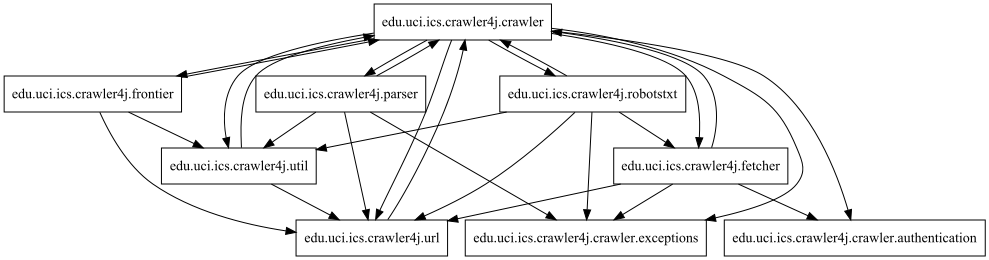
\includegraphics[scale=0.5]{img/crawler_packages_orig}
    \caption{\textit{crawler4j} sistemos struktūra}
    \label{img:crawler_packages_orig}
\end{figure}

Atlikus sistemos kokybės matų analizę galima pamatyti sistemai būdingas problemas:
\begin{center}
    \begin{tabular}{|c|c|c|c|c|c|c|c|}
        \hline
        Paketo vardas & \textit{N} & \textit{A} & \textit{E} & \textit{S} & \textit{A} & \textit{D} & \textit{C} \\ [0.5ex]
        \hline\hline
        edu.uci.ics.crawler4j.crawler.authentication & 4 & 2 & 0 & 0.0 & 0.25 & 0.75 & 0\\
        \hline
        edu.uci.ics.crawler4j.url & 4 & 6 & 1 & 0.143 & 0.0 & 0.857 & 1 \\
        \hline
        edu.uci.ics.crawler4j.crawler.exceptions & 3 & 4 & 0 & 0.0 & 0.0 & 1.0 & 0\\
        \hline
        edu.uci.ics.crawler4j.crawler & 5 & 6 & 8 & 0.571 & 0.2 & 0.229 & 5 \\
        \hline
        edu.uci.ics.crawler4j.robotstxt & 6 & 1 & 5 & 0.833 & 0.0 & 0.167 & 1 \\
        \hline
        edu.uci.ics.crawler4j.frontier & 6 & 1 & 3 & 0.75 & 0.0 & 0.25 & 1 \\
        \hline
        edu.uci.ics.crawler4j.fetcher & 6 & 2 & 4 & 0.667 & 0.0 & 0.333 & 1 \\
        \hline
        edu.uci.ics.crawler4j.util & 3 & 4 & 2 & 0.333 & 0.0 & 0.667 & 0 \\
        \hline
        edu.uci.ics.crawler4j.parser & 12 & 1 & 4 & 0.8 & 0.167 & 0.033 & 1 \\
        \hline
    \end{tabular}
    \begin{tabular}{|c|c|c|c|c|c|c|}
        \hline
        $\bar{N}$ & $\bar{A}$ & $\bar{E}$ & $\bar{S}$ & $\bar{A}$ & $\bar{D}$ & $sum(C)$ \\ [0.5ex]
        \hline\hline
        5 & 3 & 3 & 0.455 & 0.069 & 0.476 & 5\\
        \hline
    \end{tabular}
\end{center}
Iš bendros sistemos analizės bei matų lentelės rezultatu matomos kelios sistemos problemos -
\begin{itemize}
    \item \textbf{Problema numeris 1} - nors ši tai nesimato kokybės matuose, bet atlikus bendra sistemos kodo analizę matoma,
    kad sistemos paketuose yra daug sąsajų su skirtingais jų įgyvendinimais, todėl yra sunku
    rasti visus specifinės sąsajos įgyvendinimus, esama paketų struktūra tam negelbėja
    \item \textbf{Problema numeris 2} - paketo \textit{edu.uci.ics.crawler4j.parser} viduje yra 12 klasių, todėl sunku suprasti už kokius funkcionalumus jis atsakingas
    ir kada jį reikėtų nagrinėti bei keisti.
    \item \textbf{Problema numeris 3} - Sistema turi daug ciklinių prilausomynbių kur du arba daugiau paketų priklauso vienas nuo kito.
    Tai aiškiai matosi sistemos paketų diagramoje\ref{img:crawler_packages_orig}, ciklinėse priklausomybėse išviso dalyvauja 10 paketų ir kartu jie sudaro 5 ciklinių priklausomybių sekas,
    kurios turėtų būti pašalintos.
\end{itemize}

Sistemos paketas \textit{edu.uci.ics.crawler4j.parse}, turi sąsają \textit{ParseData} bei 4 skirtingųs jos įgyvendinimus - \textit{CssParseData, TextParseData, HtmlParseData, BinaryParseData},
šios klasės pakete dalinasi vieta dar su 9 klasėmis, todėl yra gan nepatogu rasti ieškomo paketo įgyvendinimo.
\begin{figure}[H]
    \snugshade
    \dirtree{%
        .1 {/parser} .
        .2 {AllTagMapper}.
        .2 {ParseData}.
        .3 {TextParseData}.
        .3 {HtmlParseData}.
        .2 {CssParseData}.
        .2 {BinaryParseData}.
        .2 {ExtractedUrlAnchorPair}.
        .2 {HtmlParser}.
        .2 {HtmlContentHandler}.
        .2 {TikaHtmlParser}.
        .2 {Parser}.
    }
    \endsnugshade
    \caption{\textit{parser} paketo struktūra}
\end{figure}
Šiam paketui sutvarkyti taikomas \textit{Sąsajų atskyrimo} šablonas - sąsaja iškeliama į atskirą paketą \textit{parse}, jos įgyvendinimai perkliami į minėto
paketo subpaketus.
Taip pat sukuriama \textit{ParseDataFactory} klasė, kurį grąžina tinkamą \textit{ParseData} sąsajos implementiciją, pagal nurodyta turinio tipą, paslepiant įgyvendinimo pavadinimą nuo
funkcijos naudotojo.
\begin{figure}[H]
    \begin{lstlisting}[language=Python]
public final class ParseDataFactory {

    public static ParseData parseDataOf(String contentType) {
        if (Util.hasBinaryContent(contentType)) {
            return new BinaryParseData();
        }

        if (Util.hasCssTextContent(contentType)) {
            return new CssParseData();
        }

        if (Util.hasPlainTextContent(contentType)) {
            return new TextParseData();
        }
        throw new UnsupportedContentTypeException(contentType);
    }
}
    \end{lstlisting}
    \caption{\textit{ParseDataFactory} klasė įgyvendinimas }
\end{figure}
Šie pertvarkymai pakeičią \textit{parser} paketo struktūra:
\begin{figure}[H]
    \snugshade
    \dirtree{%
        .1 {/parser} .
        .2 {parse}.
        .3 {ParseData // Sąsaja}.
        .3 {text}.
        .4 {TextParseData // Pirmas sąsajos įgyvendinimas}.
        .3 {html }.
        .4 {HtmlParseData // Antras sąsajos įgyvendinimas}.
        .3 {css }.
        .4 {CssParseData // Trečias sąsajos įgyvendinimas}.
        .3 {binary}.
        .4 {BinaryParseData // Ketvirtas sąsajos įgyvendinimas}.
        .3 {factory}.
        .4 {ParseDataFactory // Klasė grąžinanti tinkamą sąsajos įgyvendnimą}.
        .2 {ExtractedUrlAnchorPair}.
        .2 {HtmlParser}.
        .2 {HtmlContentHandler}.
        .2 {TikaHtmlParser}.
        .2 {Parser}.
    }
    \endsnugshade
    \caption{\textit{parser} paketo struktūra po pirmojo pertvarkymo}
\end{figure}
Dėl atskirtos sąsajos ir jos įgyvendinimų tampa daug paprasčiau ją rasti, bei suprasti sistemoje egzistuojančius jos įgyvendinimus.
Tokia struktūra išsprendžia sistemos \textbf{problemą numeris 1}.
Šis pertvarkymas taip išsprendė \textbf{problemą numeris 2}, sumažinant klasių skaičių pakete į 5.
Palyginus pertvarkytos ir buvusios sitemos matus matome, kad nors sistemą tapo aiškensė, tai nepadarė nesumažino paketų kokybės matų:
\begin{center}
    \begin{tabular}{|c|c|c|c|c|c|c|c|}
        \hline
        Paketas \textit{edu.uci.ics.crawler4j.parser} & \textit{N} & \textit{A} & \textit{E} & \textit{S} & \textit{A} & \textit{D} & \textit{C} \\ [0.5ex]
        \hline\hline
        Prieš pakeitimus & 12 & 1 & 4 & 0.8 & 0.167 & 0.033 & 1 \\
        \hline
        Po pakeitimų & 5 & 1 & 7 & 0.875 & 0.167 & 0.042 & 1 \\
        \hline
    \end{tabular}
    \begin{tabular}{|c|c|c|c|c|c|c|c|}
        \hline
        & $\bar{N}$ & $\bar{A}$ & $\bar{E}$ & $\bar{S}$ & $\bar{A}$ & $\bar{D}$ & $sum(C)$\\ [0.5ex]
        \hline\hline
        Prieš pakeitimus & 5 & 3 & 3 & 0.455 & 0.069 & 0.476 & 5\\
        \hline
        Po pakeitimus & 4 & 3 & 3 & 0.505 & 0.108 & 0.409 & 5 \\
        \hline
    \end{tabular}
\end{center}
Kad išspresti \textbf{problemą numeris 3} - ciklines priklausomybes, reikia identifikuoti klases, kurių priklausomybės
sudaro ciklus ir iškelti jas į atskirūs paketus.
todo: pridėti citavima iš straipsnio apie ciklinių priklausomybiu eliminavimą

Kuriant naujus paketus vadovaujamasi \textit{skirstymo pagal teikiamą funkcionalumą} šablonu, užtikrinant, kad kiekvienas
paketas teikia vieną, aiškiai apibrėžtą funkciją, kuri yra pasiekiama per pakete aprašytą sąsają.
Paketo vidus yra pasleptas su \textit{Java} kalbos pasiekiamumo modifikatoriais - konkrečių klasių negalima inicializuoti už paketo ribų,
nes jų konstruktoriai privatus.
Sąsajos įgyvendinimas gaunamas \textit{static factory} pagalba.
todo: aprašyti kas tai yra

\begin{figure}[H]
    \begin{lstlisting}[language=Python]
public interface HtmlParser {

    HtmlParseData parse(ParsedPage page, String contextURL) throws ParseException;

    // Grąžinamas sąsajos įgyvendinimas
    static HtmlParser newHtmlParser(CrawlConfig config, TLDList tldList) throws InstantiationException, IllegalAccessException  {
        return new TikaHtmlParser(config, tldList);
    }
}

// Sąsajos įgyvendinimas. Nėra viešas, pasiekiamas tik paketo viduje,
// nes klasė ir konstruktorius nenaudoja public raktažodžių
class TikaHtmlParser implements HtmlParser {
   ...
    TikaHtmlParser(CrawlConfig config, TLDList tldList) throws InstantiationException, IllegalAccessException {
     ...
    }
    \end{lstlisting}
    \caption{\textit{skirstymo pagal teikiamą funkcionalumą} šablono sąsaja}
\end{figure}
Peržiūrėjus paketus su ciklinėmis priklausomybės iš jų buvo išskirti šie nauji funkcionalumai, kuriems
buvo sukurti atskiri paketai:
\begin{itemize}
    \item Iš \textit{parser} paketo iškeltas funkcionalumas \textit{html} turiniui apdoroti, patalpintas į \textit{parser/html} paketą.
    Po šio pertvarkymo \textit{parser} paketas pasidaro pakankamai mažas turėti viena funkcionalumą - primti puslapį ir deleguoti jį apdorojimui kitai klasėi, pagal puslapio tipą.
    \item Iš \textit{robotstxt} paketo iškeltas funkcionalumas patikrinti ar sistema autorizuota apdoroti pasirinktą puslapi į \textit{robotstxt/permissions} paketą.
    \item Iš \textit{crawler} paketo iškeltas funkcionalumas, programiškai aprašantys internetinį puslapį į \textit{page} paketą.
    \item Iš \textit{crawler} paketo iškeltas funcionalumas, nustatyti įrankio konfiguraciją į \textit{config} paketą.
    \item Iš \textit{url} paketo iškeltas funcionalumas, gauti internetinių domenų pavadinimus į  \textit{tld} paketą.
\end{itemize}

\begin{figure}[H]
    \snugshade
    \dirtree{%
        .1 {/} .
        .2 {crawler4j}.
        .3 {crawler}.
        .4 {authentication}.
        .4 {exceptions}.
        .3 {fetcher}.
        .3 {frontier}.
        .3 {parser}.
        .4 {parse}.
        .5 {binary}.
        .5 {css}.
        .5 {factory}.
        .5 {html}.
        .5 {text}.
        .3 {robotstxt}.
        .3 {url}.
        .3 {util}.
    }
    \endsnugshade
    \caption{\textit{crawler4j} paketų medis prieš iškėliant minėtus funkcionalumus}
\end{figure}

\begin{figure}[H]
    \snugshade
    \dirtree{%
        .1 {/} .
        .2 {crawler4j}.
        .3 {config}.
        .3 {crawler}.
        .4 {authentication}.
        .4 {exceptions}.
        .3 {fetcher}.
        .3 {frontier}.
        .3 {page}.
        .3 {parser}.
        .4 {html}.
        .4 {parse}.
        .5 {binary}.
        .5 {css}.
        .5 {factory}.
        .5 {html}.
        .5 {text}.
        .3 {robotstxt}.
        .4 {permissions}.
        .3 {url}.
        .4 {canonicalizer}.
        .4 {tld}.
        .3 {util}.
    }
    \endsnugshade
    \caption{\textit{crawler4j} paketų medis iškėlus minėtus funkcionalumus}
\end{figure}

Atlikus šiuos funkcionalumų ištraukimus į atskirus paketus buvo panaikintos žiedinės priklausomybės.
Naujoje paketų diagramoje galime matyti, jog dabar sistema turi daug daugiau paketų, tačiau jų priklausomybių kryptys daug aiškesnės:
\subsection{\textit{Crawler} sistema}
\begin{figure}[H]
    \centering
    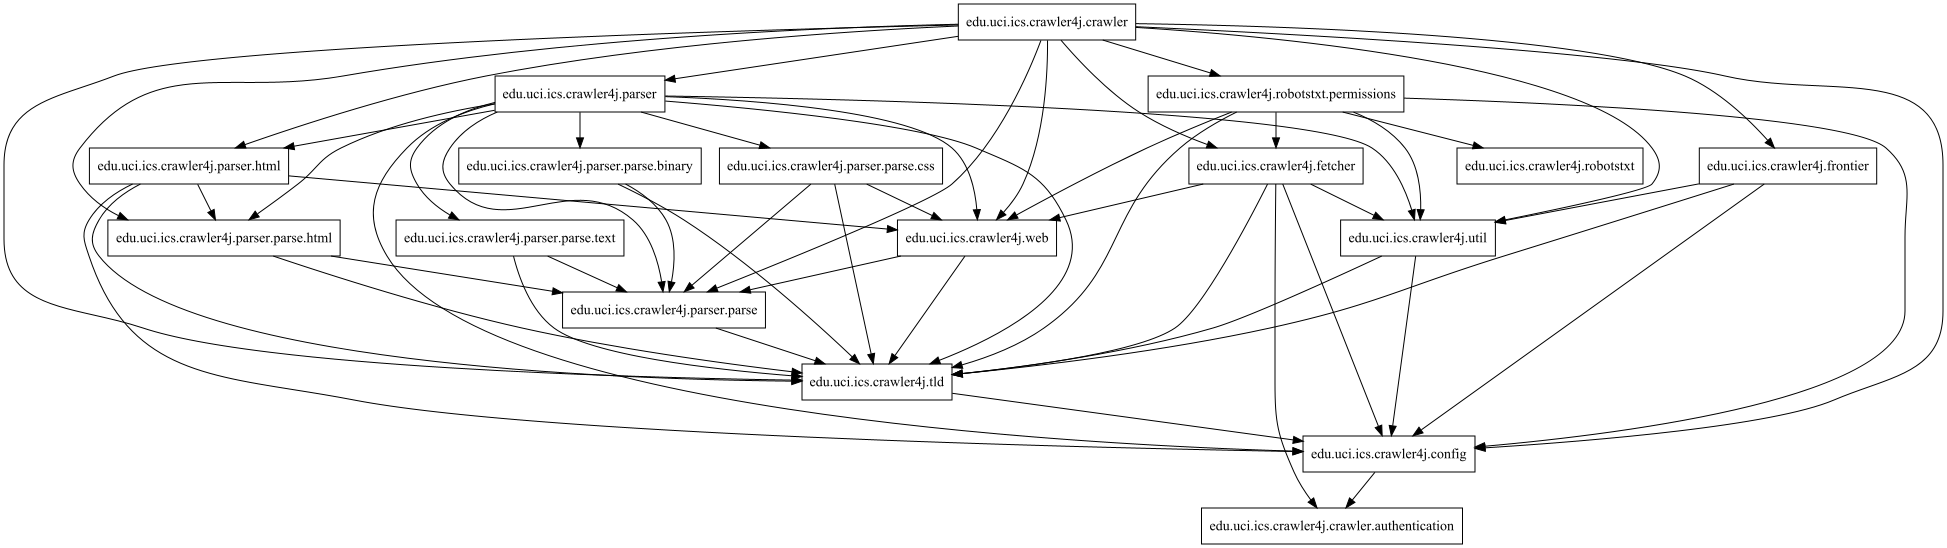
\includegraphics[scale=0.2]{img/crawler_packages_v2}
    \caption{\textit{crawler4j} sistemos struktūra po antro pertvarkymo}
    \label{img:crawler_packages_v2}
\end{figure}
todo: ranka perpaišyti sugeneruotus paveikslėlius, kad jie geriau tilptų į puslapi


Atlikus matų analizę ant naujai pertvarkytos sistemos yra matoma, kad sistemos kokybė nenukrito:
\begin{center}
    \begin{tabular}{|c|c|c|c|c|c|c|c|}
        \hline
        Paketo vardas & \textit{N} & \textit{A} & \textit{E} & \textit{S} & \textit{A} & \textit{D} & \textit{C} \\ [0.5ex]
        \hline\hline
        edu.uci.ics.crawler4j.parser.parse.binary & 1 & 1 & 2 & 0.667 & 0.0 & 0.333 & 0\\
        \hline
        edu.uci.ics.crawler4j.url & 1 & 12 & 1 & 0.077 & 0.0 & 0.923 & 0\\
        \hline
        edu.uci.ics.crawler4j.crawler.exceptions & 1 & 3 & 0 & 0.0 & 0.0 & 1.0 & 0 \\
        \hline
        edu.uci.ics.crawler4j.crawler & 4 & 0 & 13 & 1.0 & 0.25 & 0.25 & 0  \\
        \hline
        edu.uci.ics.crawler4j.parser.html & 2 & 1 & 7 & 0.875 & 0.5 & 0.375 & 0 \\
        \hline
        edu.uci.ics.crawler4j.robotstxt.permissions & 2 & 1 & 7 & 0.875 & 0.5 & 0.375 & 0\\
        \hline
        edu.uci.ics.crawler4j.config & 1 & 8 & 1 & 0.111 & 0.0 & 0.889 & 0 \\
        \hline
        edu.uci.ics.crawler4j.frontier & 6 & 1 & 3 & 0.75 & 0.0 & 0.25 & 0  \\
        \hline
        edu.uci.ics.crawler4j.page & 2 & 5 & 2 & 0.286 & 0.5 & 0.214 & 0 \\
        \hline
        edu.uci.ics.crawler4j.parser.parse.factory & 1 & 1 & 5 & 0.833 & 0.0 & 0.167 & 0 \\
        \hline
        edu.uci.ics.crawler4j.parser & 6 & 2 & 8 & 0.8 & 0.0 & 0.2 &0 \\
        \hline
        edu.uci.ics.crawler4j.crawler.authentication & 4 & 2 & 0 & 0.0 & 0.25 & 0.75 & 0 \\
        \hline
        edu.uci.ics.crawler4j.parser.parse.css & 1 & 1 & 3 & 0.75 & 0.0 & 0.25 & 0\\
        \hline
        edu.uci.ics.crawler4j.robotstxt & 5 & 1 & 0 & 0.0 & 0.0 & 1.0 & 0 \\
        \hline
        edu.uci.ics.crawler4j.url.tld & 2 & 5 & 1 & 0.167 & 0.5 & 0.333 & 0 \\
        \hline
        edu.uci.ics.crawler4j.parser.parse.html & 1 & 3 & 2 & 0.4 & 0.0 & 0.6 & 0\\
        \hline
        edu.uci.ics.crawler4j.parser.parse & 1 & 8 & 1 & 0.111 & 1.0 & 0.111 & 0 \\
        \hline
        edu.uci.ics.crawler4j.fetcher & 6 & 2 & 6 & 0.75 & 0.0 & 0.25 & 0 \\
        \hline
        edu.uci.ics.crawler4j.util & 3 & 5 & 3 & 0.375 & 0.0 & 0.625 & 0 \\
        \hline
        edu.uci.ics.crawler4j.parser.parse.text & 1 & 1 & 2 & 0.667 & 0.0 & 0.333 & 0 \\
        \hline
        edu.uci.ics.crawler4j.url.canonicalizer & 3 & 4 & 0 & 0.0 & 0.333 & 0.667 & 0 \\
        \hline
    \end{tabular}
    \begin{tabular}{|c|c|c|c|c|c|c|c|}
        \hline
        & $\bar{N}$ & $\bar{A}$ & $\bar{E}$ & $\bar{S}$ & $\bar{A}$ & $\bar{D}$ & $sum(C)$\\ [0.5ex]
        \hline\hline
        Prieš pakeitimus & 5 & 3 & 3 & 0.455 & 0.069 & 0.476 & 5\\
        \hline
        Po pirmos iteracijos & 4 & 3 & 3 & 0.505 & 0.108 & 0.409 & 5 \\
        \hline
        Po visų pakeitimų & 3 & 3 & 3 & 0.452 & 0.183 & 0.471 & 0 \\
        \hline
    \end{tabular}
\end{center}
Todėl po šio pertvarkymo galima teigti, kad šablonai \textit{skirstymas pagal teikiamą funkcionalumą} ir \textit{sąsajų atskyrimas}, išsprendė visas 3 sistemoje matytas problemas,
padarė sistemą lengviau suprantamą žmogui, panaikino ciklinės priklausomybes bet taip pat neturėjo neigiamos įtakos matams, nurodantiems
sistemos įgyvendinimo kokybę.

todo: parašyti, pertvarkymo tikslas nėra gerinti matus, o jie yra naudojami tik tam kad isitikinti, jog kokybė nesuprastejo. Svarbiau skaitomumas, o ne kokybė paremta matais
todo: prideti figures prie lenteliu